%-----------------------------------------------------------------
%	BOOTSTRAP: DISTRIBUTIONAL PROPERTIES OF THE DATA
%	!TEX root = ./../main.tex
%-----------------------------------------------------------------
\subsection{Distributional properties of the data}\label{sec:distribution-analysis}
It is important to notice that the relationships between a storm's $PDI$ and its lifetime are of non-linear nature. This naturally means that our regressions need to follow a so-called log--log model:
\begin{align}\label{eq:lm-model-bis}
	\log \Psi = \beta_{0} + \beta_{1} \log \Phi + \epsilon,
	\tag{\ref{eq:lm-model} bis}
\end{align}
where $\log \Psi \equiv Y$ and $\log \Phi \equiv X$.

We do not know exactly how the $PDI$ and the lifetime of the storms are exactly correlated; we just suspect there is a correlation. For this reason, we not only compute the $Y(X)$ fit for each data set, but also $X(Y) = \hat{\beta}_{0} + \hat{\beta}_{1} Y$, which is calculated as stated in \cref{sec:lm-coefs} just interchanging the role of $X$ and $Y$.

\medskip
Before performing the regression analysis we should study, however, the bivariate distribution of the data and the marginal distributions of the $PDI$ and the lifetime of storms to see any difference between the two populations that are result of the separation of the storms by SST class.

%-----------------------------------------------------------------
\subsubsection{Bivariate lognormal distribution}\label{sec:bvln-distribution}
\nocite{Thomopoulos2017}
The bivariate lognormal has two variables, $X_{1}$ and $X_{2}$, that are jointly related, and has five parameters, $\mu_{1}$, $\mu_{2}$, $\sigma_{1}^{2}$, $\sigma_{2}^{2}$, and $r$:
\begin{align}
	f(X_{1}, X_{2}) \sim \mc{BVLN}(\mu_{1}, \mu_{2}, \sigma_{1}^{2}, \sigma_{2}^{2}, r).
\end{align}

The marginal distributions are lognormally distributed, i.e., the logarithm of them is normally distributed:
\begin{align}
	\log X_{1} \sim \mc{N}(\mu_{1}, \sigma_{1}^{2})
	\qc
	\log X_{2} \sim \mc{N}(\mu_{2}, \sigma_{2}^{2})
	,
\end{align}
and when the value of one of the variables is known, the distribution on the other is also normally distributed. This, naturally implies that the joint distribution of the logarithm of the variables follows a bivariate normal distribution:
\begin{align}
	f(\log X_{1}, \log X_{2}) \sim \mc{BVN}(\mu_{1}, \mu_{2}, \sigma_{1}^{2}, \sigma_{2}^{2}, r) .
\end{align}

\Cref{fig:bvn-example} shows a bivariate normal distribution to illustrate both the joint distribution between the two variables $X_{1}$ and $X_{2}$ and their respective marginal distributions.
\begin{figure}[H]
	\centering
	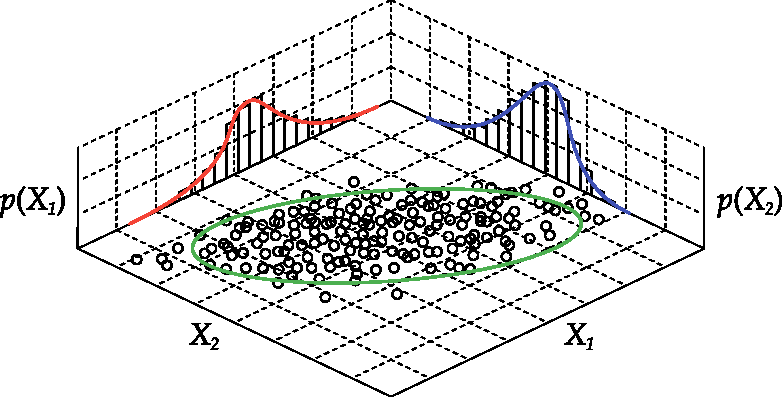
\includegraphics[width=0.75\textwidth]{images/bvn-example}
	\caption{Bivariate normal distribution $f(X_{1}, X_{2})$ and the marginal distributions of $X_{1}$ and $X_{2}$}
	\label{fig:bvn-example}
\end{figure}

% \medskip
In \Cref{fig:natl-bvln} and \Cref{fig:epac-bvln} we can see the bivariate lognormal distributions of the $PDI$ and lifetime of the storms for the North Atlantic and Northeast Pacific basins separating storms by SST class.

\begin{figure}[H]
	\centering
	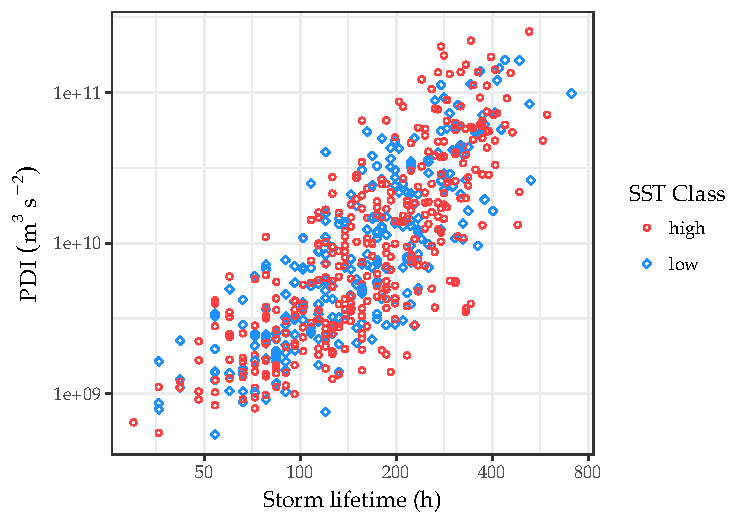
\includegraphics[width=0.8\textwidth]{images/natl-bvln}
	\caption{Bivariate lognormal distribution $f(PDI, \text{lifetime})$ of the hurricane observations for the North Atlantic basin}
	\label{fig:natl-bvln}
\end{figure}

\begin{figure}[H]
	\centering
	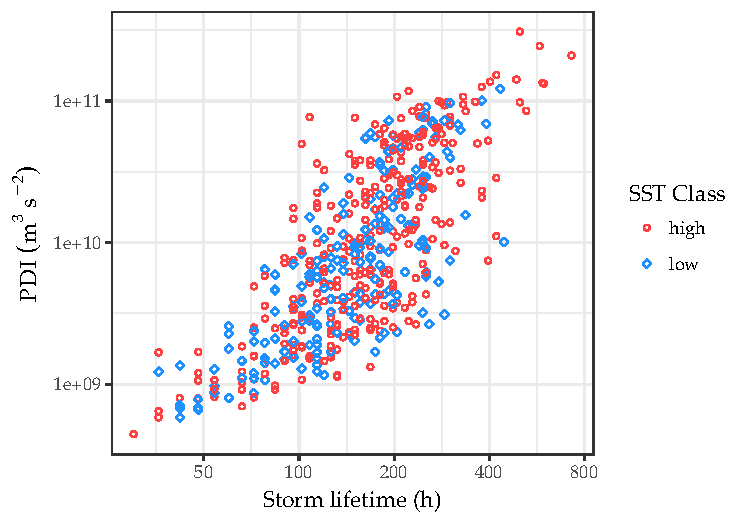
\includegraphics[width=0.8\textwidth]{images/epac-bvln}
	\caption{Bivariate lognormal distribution $f(PDI, \text{lifetime})$ of the hurricane observations for the Northeast Pacific basin}
	\label{fig:epac-bvln}
\end{figure}

The first thing to notice is that, as our hypothesis predicts, although the joint distributions seem to overlap, the expected value $(\mu_{PDI}, \mu_{\text{lifetime}})$ seems to be different for the distributions associated to each SST class. To see this more clearly, we should perform a descriptive univariate analysis of the marginal distributions.

%-----------------------------------------------------------------
% \newpage
\subsubsection{Descriptive univariate analysis of the marginals}\label{ssec:univariate}

% \todo[inline]{Show that we care about the expected values, not the distributions themselves. If possible, add $t$ test to compare them}

In \Cref{fig:natl-marginals-pdi} and \Cref{fig:natl-marginals-lifetime} we can see the marginal distributions of the $PDI$ and lifetime, in logarithmic scale, for the North Atlantic basin data, separating the data by SST class. For the marginal analysis we also show the expected value $\mu$ as a dashed line. Similarly, in \Cref{fig:epac-marginals-pdi} and \Cref{fig:epac-marginals-lifetime} we show the same marginal distributions for the Northeast Pacific basin data.

A statistical summary of the marginals for both basins can be seen in \Cref{tab:natl-marginals-stats} and \Cref{tab:epac-marginals-stats}.

\medskip
We can see that the marginals do not follow exactly a normal distribution for the $PDI$. This is expected, as \textcite{Corral2010} show that the $PDI$ distributions can be characterised by a power-law decay in their central regions. The lifetime marginal distributions do, as it is expected from a bivariate lognormal distribution, roughly follow a normal distribution.

The results show that the expected value $(\mu_{PDI}, \mu_{\text{lifetime}})$ of the joint distributions are displaced to the right-upper corner for high-SST years. This can be clearly seen in the fact that high-SST years have a longer right tail on account of having more available energy from the sea, and as a result displace the mean of the population $\mu$ to higher values as well. This is both reflected in the $PDI$ and the storm lifetime.

 % are not the same for storms occurred in low-SST years and high-SST years, but the expected values for the high-SST years are higher, supporting our hypothesis that high-SST years should have a longer right tail on account of having more available energy from the sea, displacing the expected value $(\mu_{PDI}, \mu_{\text{lifetime}})$ of the joint distribution to the upper-right corner.

\begin{figure}[H]
	\centering
	\subfloat[Marginal distribution of the $PDI$]{%
		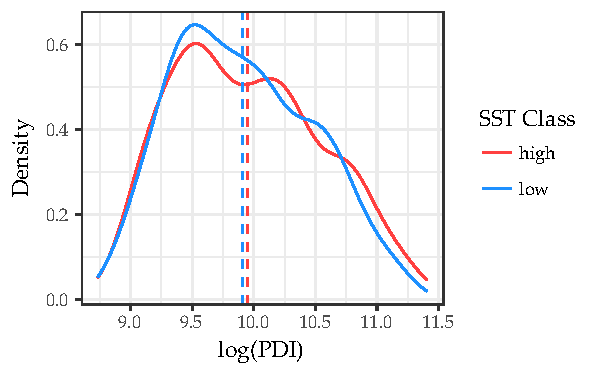
\includegraphics[width=0.5\textwidth]{./images/natl-marginals-pdi}
		\label{fig:natl-marginals-pdi}%
		}%
	\subfloat[Marginal distribution of the lifetime]{%
		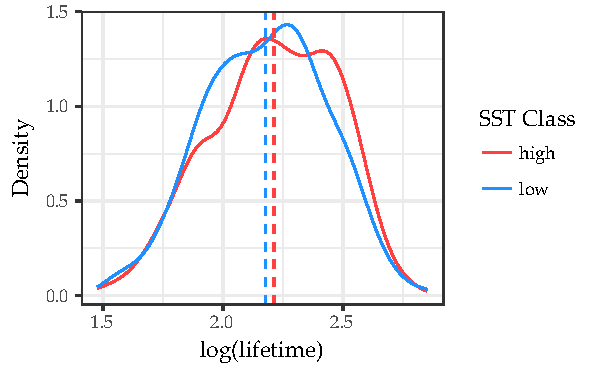
\includegraphics[width=0.5\textwidth]{./images/natl-marginals-lifetime}
		\label{fig:natl-marginals-lifetime}%
		}%
	\caption{Marginal analysis for the variables of the bivariate lognormal distribution for the North Atlantic basin data}
	\label{fig:natl-marginals}
\end{figure}

\vspace{-5pt}
\begin{table}[H]
	\centering
	\begin{tabular}{lccc}
		\toprule
		\toprule
		Marginal variable & Data & Mean $\mu$            & Median \\
		\midrule
		\multirow{2}{*}{$\log(PDI)$}
		 & Low-SST               & \num{9.91 \pm 0.04} & \num{9.86 \pm 0.04} \\
		 & High-SST              & \num{9.95 \pm 0.03} & \num{9.91 \pm 0.04} \\
		\midrule
		% \cmidrule(l){2-5}
		\multirow{2}{*}{$\log(\text{lifetime})$}
		 & Low-SST               & \num{2.18 \pm 0.02} & \num{2.19 \pm 0.02} \\
		 & High-SST              & \num{2.21 \pm 0.01} & \num{2.23 \pm 0.02} \\
		\bottomrule
	\end{tabular}
	\caption{Statistical summary for the low-SST and high-SST subsets of the marginals of the bivariate lognormal distribution for the North Atlantic basin data}
	\label{tab:natl-marginals-stats}
\end{table}

\vspace{-5pt}
\begin{figure}[H]
	\centering
	\subfloat[Marginal distribution of the $PDI$]{%
		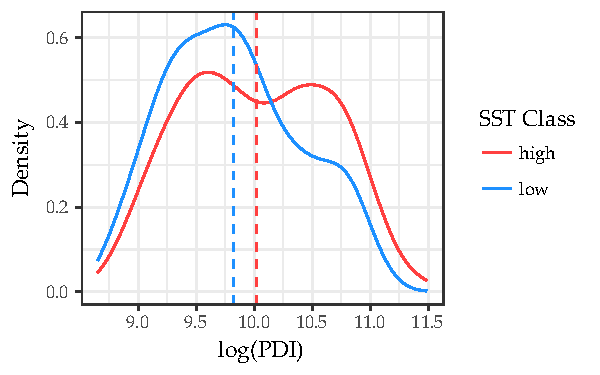
\includegraphics[width=0.5\textwidth]{./images/epac-marginals-pdi}
		\label{fig:epac-marginals-pdi}%
		}%
	\subfloat[Marginal distribution of the lifetime]{%
		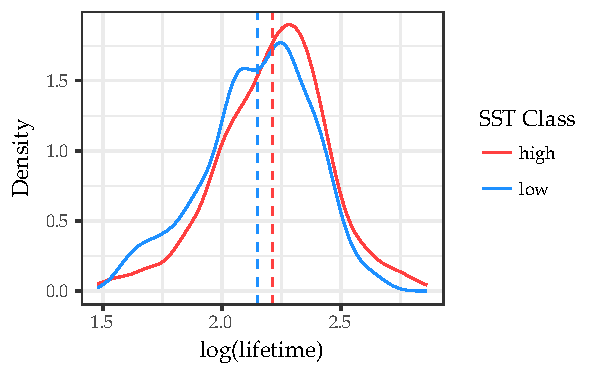
\includegraphics[width=0.5\textwidth]{./images/epac-marginals-lifetime}
		\label{fig:epac-marginals-lifetime}%
		}%
	\caption{Marginal analysis for the variables of the bivariate lognormal distribution for the Northeast Pacific basin data}
	\label{fig:epac-marginals}
\end{figure}


\begin{table}[H]
	\centering
	\begin{tabular}{clcc}
		\toprule
		\toprule
		Marginal variable & Data & Mean $\mu$            & Median \\
		\midrule
		\multirow{2}{*}{$\log(PDI)$}
		 & Low-SST               & \num{9.82 \pm 0.04} & \num{9.78 \pm 0.05} \\
		 & High-SST              & \num{10.0 \pm 0.04} & \num{9.99 \pm 0.04} \\
		\midrule
		% \cmidrule(l){2-5}
		\multirow{2}{*}{$\log(\text{lifetime})$}
		 & Low-SST               & \num{2.15 \pm 0.02} & \num{2.18 \pm 0.02} \\
		 & High-SST              & \num{2.21 \pm 0.01} & \num{2.23 \pm 0.02} \\
		\bottomrule
	\end{tabular}
	\caption{Statistical summary for the low-SST and high-SST subsets of the marginals of the bivariate lognormal distribution for the Northeast Pacific basin data}
	\label{tab:epac-marginals-stats}
\end{table}



% \num{9.91 \pm 0.0351} & \num{9.86 \pm 0.0440}
% \num{9.95 \pm 0.0322} & \num{9.91 \pm 0.0403}

% \num{2.18 \pm 0.0157} & \num{2.19 \pm 0.0197}
% \num{2.21 \pm 0.0138} & \num{2.23 \pm 0.0173}

% \num{9.82 \pm 0.0411} & \num{9.78 \pm 0.0516}
% \num{10.0 \pm 0.0355} & \num{9.99 \pm 0.0445}

% \num{2.15 \pm 0.0162} & \num{2.18 \pm 0.0203}
% \num{2.21 \pm 0.0130} & \num{2.23 \pm 0.0162}
